% Created by tikzDevice version 0.7.0 on 2015-01-08 14:52:44
% !TEX encoding = UTF-8 Unicode
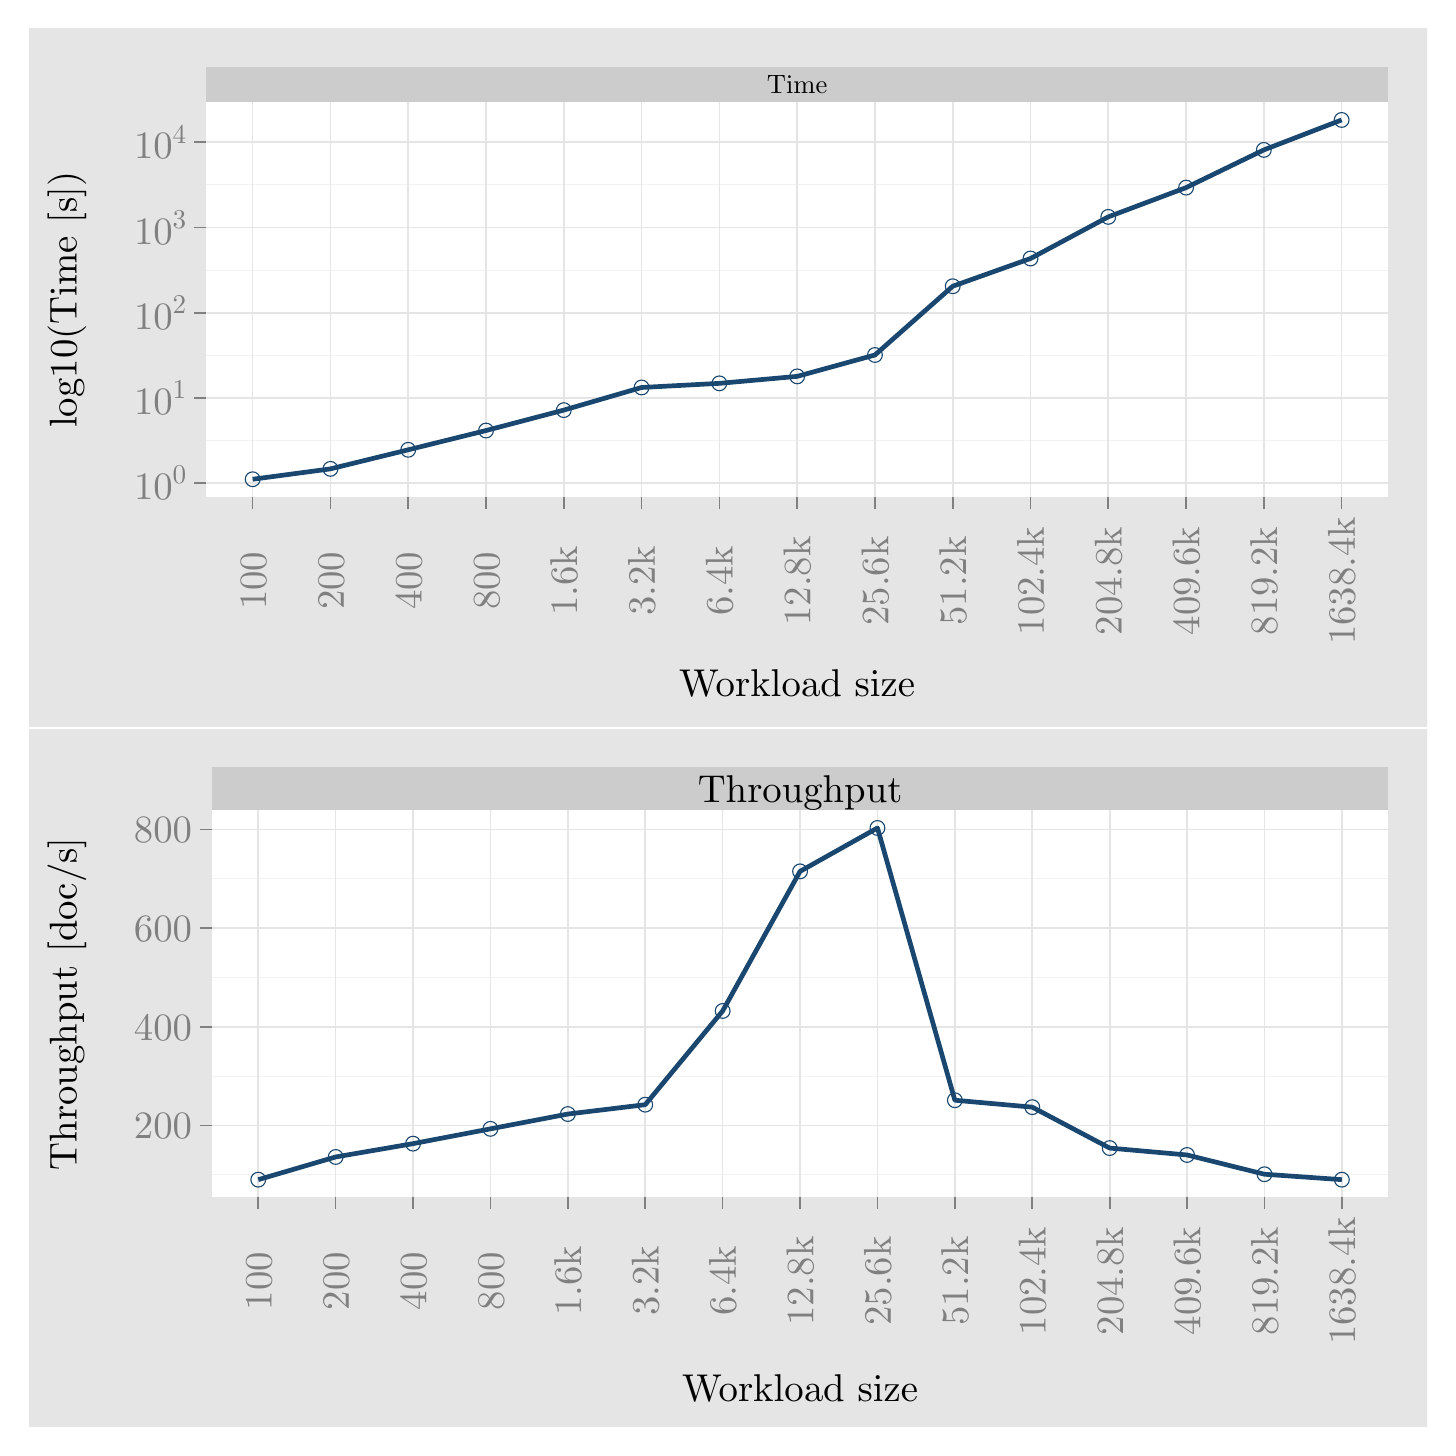
\begin{tikzpicture}[x=1pt,y=1pt]
\definecolor[named]{fillColor}{rgb}{1.00,1.00,1.00}
\path[use as bounding box,fill=fillColor,fill opacity=0.00] (0,0) rectangle (505.89,505.89);
\begin{scope}
\path[clip] (  0.00,252.94) rectangle (505.89,505.89);
\definecolor[named]{drawColor}{rgb}{1.00,1.00,1.00}
\definecolor[named]{fillColor}{rgb}{0.90,0.90,0.90}

\path[draw=drawColor,line width= 0.6pt,line join=round,line cap=round,fill=fillColor] (  0.00,252.94) rectangle (505.89,505.89);
\end{scope}
\begin{scope}
\path[clip] ( 64.44,336.22) rectangle (491.66,479.03);
\definecolor[named]{fillColor}{rgb}{1.00,1.00,1.00}

\path[fill=fillColor] ( 64.44,336.22) rectangle (491.66,479.03);
\definecolor[named]{drawColor}{rgb}{0.95,0.95,0.95}

\path[draw=drawColor,line width= 0.3pt,line join=round] ( 64.44,356.71) --
	(491.66,356.71);

\path[draw=drawColor,line width= 0.3pt,line join=round] ( 64.44,387.50) --
	(491.66,387.50);

\path[draw=drawColor,line width= 0.3pt,line join=round] ( 64.44,418.29) --
	(491.66,418.29);

\path[draw=drawColor,line width= 0.3pt,line join=round] ( 64.44,449.09) --
	(491.66,449.09);
\definecolor[named]{drawColor}{rgb}{0.90,0.90,0.90}

\path[draw=drawColor,line width= 0.6pt,line join=round] ( 64.44,341.31) --
	(491.66,341.31);

\path[draw=drawColor,line width= 0.6pt,line join=round] ( 64.44,372.10) --
	(491.66,372.10);

\path[draw=drawColor,line width= 0.6pt,line join=round] ( 64.44,402.90) --
	(491.66,402.90);

\path[draw=drawColor,line width= 0.6pt,line join=round] ( 64.44,433.69) --
	(491.66,433.69);

\path[draw=drawColor,line width= 0.6pt,line join=round] ( 64.44,464.48) --
	(491.66,464.48);

\path[draw=drawColor,line width= 0.6pt,line join=round] ( 81.30,336.22) --
	( 81.30,479.03);

\path[draw=drawColor,line width= 0.6pt,line join=round] (109.41,336.22) --
	(109.41,479.03);

\path[draw=drawColor,line width= 0.6pt,line join=round] (137.51,336.22) --
	(137.51,479.03);

\path[draw=drawColor,line width= 0.6pt,line join=round] (165.62,336.22) --
	(165.62,479.03);

\path[draw=drawColor,line width= 0.6pt,line join=round] (193.73,336.22) --
	(193.73,479.03);

\path[draw=drawColor,line width= 0.6pt,line join=round] (221.84,336.22) --
	(221.84,479.03);

\path[draw=drawColor,line width= 0.6pt,line join=round] (249.94,336.22) --
	(249.94,479.03);

\path[draw=drawColor,line width= 0.6pt,line join=round] (278.05,336.22) --
	(278.05,479.03);

\path[draw=drawColor,line width= 0.6pt,line join=round] (306.16,336.22) --
	(306.16,479.03);

\path[draw=drawColor,line width= 0.6pt,line join=round] (334.26,336.22) --
	(334.26,479.03);

\path[draw=drawColor,line width= 0.6pt,line join=round] (362.37,336.22) --
	(362.37,479.03);

\path[draw=drawColor,line width= 0.6pt,line join=round] (390.48,336.22) --
	(390.48,479.03);

\path[draw=drawColor,line width= 0.6pt,line join=round] (418.59,336.22) --
	(418.59,479.03);

\path[draw=drawColor,line width= 0.6pt,line join=round] (446.69,336.22) --
	(446.69,479.03);

\path[draw=drawColor,line width= 0.6pt,line join=round] (474.80,336.22) --
	(474.80,479.03);
\definecolor[named]{drawColor}{rgb}{0.10,0.28,0.44}

\path[draw=drawColor,line width= 1.7pt,line join=round] ( 81.30,342.71) --
	(109.41,346.46) --
	(137.51,353.35) --
	(165.62,360.31) --
	(193.73,367.69) --
	(221.84,375.87) --
	(249.94,377.36) --
	(278.05,379.88) --
	(306.16,387.61) --
	(334.26,412.45) --
	(362.37,422.47) --
	(390.48,437.52) --
	(418.59,448.09) --
	(446.69,461.72) --
	(474.80,472.54);

\path[draw=drawColor,line width= 0.4pt,line join=round,line cap=round] ( 81.30,342.71) circle (  2.67);

\path[draw=drawColor,line width= 0.4pt,line join=round,line cap=round] (109.41,346.46) circle (  2.67);

\path[draw=drawColor,line width= 0.4pt,line join=round,line cap=round] (137.51,353.35) circle (  2.67);

\path[draw=drawColor,line width= 0.4pt,line join=round,line cap=round] (165.62,360.31) circle (  2.67);

\path[draw=drawColor,line width= 0.4pt,line join=round,line cap=round] (193.73,367.69) circle (  2.67);

\path[draw=drawColor,line width= 0.4pt,line join=round,line cap=round] (221.84,375.87) circle (  2.67);

\path[draw=drawColor,line width= 0.4pt,line join=round,line cap=round] (249.94,377.36) circle (  2.67);

\path[draw=drawColor,line width= 0.4pt,line join=round,line cap=round] (278.05,379.88) circle (  2.67);

\path[draw=drawColor,line width= 0.4pt,line join=round,line cap=round] (306.16,387.61) circle (  2.67);

\path[draw=drawColor,line width= 0.4pt,line join=round,line cap=round] (334.26,412.45) circle (  2.67);

\path[draw=drawColor,line width= 0.4pt,line join=round,line cap=round] (362.37,422.47) circle (  2.67);

\path[draw=drawColor,line width= 0.4pt,line join=round,line cap=round] (390.48,437.52) circle (  2.67);

\path[draw=drawColor,line width= 0.4pt,line join=round,line cap=round] (418.59,448.09) circle (  2.67);

\path[draw=drawColor,line width= 0.4pt,line join=round,line cap=round] (446.69,461.72) circle (  2.67);

\path[draw=drawColor,line width= 0.4pt,line join=round,line cap=round] (474.80,472.54) circle (  2.67);
\end{scope}
\begin{scope}
\path[clip] (  0.00,  0.00) rectangle (505.89,505.89);
\definecolor[named]{fillColor}{rgb}{0.80,0.80,0.80}

\path[fill=fillColor] ( 64.44,479.03) rectangle (491.66,491.66);
\definecolor[named]{drawColor}{rgb}{0.00,0.00,0.00}

\node[text=drawColor,anchor=base,inner sep=0pt, outer sep=0pt, scale=  0.96] at (278.05,482.04) {Time};
\end{scope}
\begin{scope}
\path[clip] (  0.00,  0.00) rectangle (505.89,505.89);
\definecolor[named]{drawColor}{rgb}{0.50,0.50,0.50}

\node[text=drawColor,anchor=base west,inner sep=0pt, outer sep=0pt, scale=  1.40] at ( 38.43,335.31) {10};

\node[text=drawColor,anchor=base west,inner sep=0pt, outer sep=0pt, scale=  0.98] at ( 52.42,341.03) {0};

\node[text=drawColor,anchor=base west,inner sep=0pt, outer sep=0pt, scale=  1.40] at ( 38.43,366.10) {10};

\node[text=drawColor,anchor=base west,inner sep=0pt, outer sep=0pt, scale=  0.98] at ( 52.42,371.82) {1};

\node[text=drawColor,anchor=base west,inner sep=0pt, outer sep=0pt, scale=  1.40] at ( 38.43,396.89) {10};

\node[text=drawColor,anchor=base west,inner sep=0pt, outer sep=0pt, scale=  0.98] at ( 52.42,402.62) {2};

\node[text=drawColor,anchor=base west,inner sep=0pt, outer sep=0pt, scale=  1.40] at ( 38.43,427.68) {10};

\node[text=drawColor,anchor=base west,inner sep=0pt, outer sep=0pt, scale=  0.98] at ( 52.42,433.41) {3};

\node[text=drawColor,anchor=base west,inner sep=0pt, outer sep=0pt, scale=  1.40] at ( 38.43,458.48) {10};

\node[text=drawColor,anchor=base west,inner sep=0pt, outer sep=0pt, scale=  0.98] at ( 52.42,464.20) {4};
\end{scope}
\begin{scope}
\path[clip] (  0.00,  0.00) rectangle (505.89,505.89);
\definecolor[named]{drawColor}{rgb}{0.50,0.50,0.50}

\path[draw=drawColor,line width= 0.6pt,line join=round] ( 60.17,341.31) --
	( 64.44,341.31);

\path[draw=drawColor,line width= 0.6pt,line join=round] ( 60.17,372.10) --
	( 64.44,372.10);

\path[draw=drawColor,line width= 0.6pt,line join=round] ( 60.17,402.90) --
	( 64.44,402.90);

\path[draw=drawColor,line width= 0.6pt,line join=round] ( 60.17,433.69) --
	( 64.44,433.69);

\path[draw=drawColor,line width= 0.6pt,line join=round] ( 60.17,464.48) --
	( 64.44,464.48);
\end{scope}
\begin{scope}
\path[clip] (  0.00,  0.00) rectangle (505.89,505.89);
\definecolor[named]{drawColor}{rgb}{0.50,0.50,0.50}

\path[draw=drawColor,line width= 0.6pt,line join=round] ( 81.30,331.95) --
	( 81.30,336.22);

\path[draw=drawColor,line width= 0.6pt,line join=round] (109.41,331.95) --
	(109.41,336.22);

\path[draw=drawColor,line width= 0.6pt,line join=round] (137.51,331.95) --
	(137.51,336.22);

\path[draw=drawColor,line width= 0.6pt,line join=round] (165.62,331.95) --
	(165.62,336.22);

\path[draw=drawColor,line width= 0.6pt,line join=round] (193.73,331.95) --
	(193.73,336.22);

\path[draw=drawColor,line width= 0.6pt,line join=round] (221.84,331.95) --
	(221.84,336.22);

\path[draw=drawColor,line width= 0.6pt,line join=round] (249.94,331.95) --
	(249.94,336.22);

\path[draw=drawColor,line width= 0.6pt,line join=round] (278.05,331.95) --
	(278.05,336.22);

\path[draw=drawColor,line width= 0.6pt,line join=round] (306.16,331.95) --
	(306.16,336.22);

\path[draw=drawColor,line width= 0.6pt,line join=round] (334.26,331.95) --
	(334.26,336.22);

\path[draw=drawColor,line width= 0.6pt,line join=round] (362.37,331.95) --
	(362.37,336.22);

\path[draw=drawColor,line width= 0.6pt,line join=round] (390.48,331.95) --
	(390.48,336.22);

\path[draw=drawColor,line width= 0.6pt,line join=round] (418.59,331.95) --
	(418.59,336.22);

\path[draw=drawColor,line width= 0.6pt,line join=round] (446.69,331.95) --
	(446.69,336.22);

\path[draw=drawColor,line width= 0.6pt,line join=round] (474.80,331.95) --
	(474.80,336.22);
\end{scope}
\begin{scope}
\path[clip] (  0.00,  0.00) rectangle (505.89,505.89);
\definecolor[named]{drawColor}{rgb}{0.50,0.50,0.50}

\node[text=drawColor,rotate= 90.00,anchor=base,inner sep=0pt, outer sep=0pt, scale=  1.40] at ( 86.12,305.97) {100};

\node[text=drawColor,rotate= 90.00,anchor=base,inner sep=0pt, outer sep=0pt, scale=  1.40] at (114.23,305.97) {200};

\node[text=drawColor,rotate= 90.00,anchor=base,inner sep=0pt, outer sep=0pt, scale=  1.40] at (142.33,305.97) {400};

\node[text=drawColor,rotate= 90.00,anchor=base,inner sep=0pt, outer sep=0pt, scale=  1.40] at (170.44,305.97) {800};

\node[text=drawColor,rotate= 90.00,anchor=base,inner sep=0pt, outer sep=0pt, scale=  1.40] at (198.55,305.97) {1.6k};

\node[text=drawColor,rotate= 90.00,anchor=base,inner sep=0pt, outer sep=0pt, scale=  1.40] at (226.66,305.97) {3.2k};

\node[text=drawColor,rotate= 90.00,anchor=base,inner sep=0pt, outer sep=0pt, scale=  1.40] at (254.76,305.97) {6.4k};

\node[text=drawColor,rotate= 90.00,anchor=base,inner sep=0pt, outer sep=0pt, scale=  1.40] at (282.87,305.97) {12.8k};

\node[text=drawColor,rotate= 90.00,anchor=base,inner sep=0pt, outer sep=0pt, scale=  1.40] at (310.98,305.97) {25.6k};

\node[text=drawColor,rotate= 90.00,anchor=base,inner sep=0pt, outer sep=0pt, scale=  1.40] at (339.08,305.97) {51.2k};

\node[text=drawColor,rotate= 90.00,anchor=base,inner sep=0pt, outer sep=0pt, scale=  1.40] at (367.19,305.97) {102.4k};

\node[text=drawColor,rotate= 90.00,anchor=base,inner sep=0pt, outer sep=0pt, scale=  1.40] at (395.30,305.97) {204.8k};

\node[text=drawColor,rotate= 90.00,anchor=base,inner sep=0pt, outer sep=0pt, scale=  1.40] at (423.41,305.97) {409.6k};

\node[text=drawColor,rotate= 90.00,anchor=base,inner sep=0pt, outer sep=0pt, scale=  1.40] at (451.51,305.97) {819.2k};

\node[text=drawColor,rotate= 90.00,anchor=base,inner sep=0pt, outer sep=0pt, scale=  1.40] at (479.62,305.97) {1638.4k};
\end{scope}
\begin{scope}
\path[clip] (  0.00,  0.00) rectangle (505.89,505.89);
\definecolor[named]{drawColor}{rgb}{0.00,0.00,0.00}

\node[text=drawColor,anchor=base,inner sep=0pt, outer sep=0pt, scale=  1.40] at (278.05,264.16) {Workload size};
\end{scope}
\begin{scope}
\path[clip] (  0.00,  0.00) rectangle (505.89,505.89);
\definecolor[named]{drawColor}{rgb}{0.00,0.00,0.00}

\node[text=drawColor,rotate= 90.00,anchor=base,inner sep=0pt, outer sep=0pt, scale=  1.40] at ( 17.70,407.62) {log10(Time [s])};
\end{scope}
\begin{scope}
\path[clip] (  0.00,  0.00) rectangle (505.89,252.94);
\definecolor[named]{drawColor}{rgb}{1.00,1.00,1.00}
\definecolor[named]{fillColor}{rgb}{0.90,0.90,0.90}

\path[draw=drawColor,line width= 0.6pt,line join=round,line cap=round,fill=fillColor] (  0.00,  0.00) rectangle (505.89,252.94);
\end{scope}
\begin{scope}
\path[clip] ( 66.53, 83.27) rectangle (491.66,223.05);
\definecolor[named]{fillColor}{rgb}{1.00,1.00,1.00}

\path[fill=fillColor] ( 66.53, 83.27) rectangle (491.66,223.05);
\definecolor[named]{drawColor}{rgb}{0.95,0.95,0.95}

\path[draw=drawColor,line width= 0.3pt,line join=round] ( 66.53, 91.41) --
	(491.66, 91.41);

\path[draw=drawColor,line width= 0.3pt,line join=round] ( 66.53,127.05) --
	(491.66,127.05);

\path[draw=drawColor,line width= 0.3pt,line join=round] ( 66.53,162.70) --
	(491.66,162.70);

\path[draw=drawColor,line width= 0.3pt,line join=round] ( 66.53,198.34) --
	(491.66,198.34);
\definecolor[named]{drawColor}{rgb}{0.90,0.90,0.90}

\path[draw=drawColor,line width= 0.6pt,line join=round] ( 66.53,109.23) --
	(491.66,109.23);

\path[draw=drawColor,line width= 0.6pt,line join=round] ( 66.53,144.87) --
	(491.66,144.87);

\path[draw=drawColor,line width= 0.6pt,line join=round] ( 66.53,180.52) --
	(491.66,180.52);

\path[draw=drawColor,line width= 0.6pt,line join=round] ( 66.53,216.17) --
	(491.66,216.17);

\path[draw=drawColor,line width= 0.6pt,line join=round] ( 83.32, 83.27) --
	( 83.32,223.05);

\path[draw=drawColor,line width= 0.6pt,line join=round] (111.29, 83.27) --
	(111.29,223.05);

\path[draw=drawColor,line width= 0.6pt,line join=round] (139.25, 83.27) --
	(139.25,223.05);

\path[draw=drawColor,line width= 0.6pt,line join=round] (167.22, 83.27) --
	(167.22,223.05);

\path[draw=drawColor,line width= 0.6pt,line join=round] (195.19, 83.27) --
	(195.19,223.05);

\path[draw=drawColor,line width= 0.6pt,line join=round] (223.16, 83.27) --
	(223.16,223.05);

\path[draw=drawColor,line width= 0.6pt,line join=round] (251.13, 83.27) --
	(251.13,223.05);

\path[draw=drawColor,line width= 0.6pt,line join=round] (279.10, 83.27) --
	(279.10,223.05);

\path[draw=drawColor,line width= 0.6pt,line join=round] (307.07, 83.27) --
	(307.07,223.05);

\path[draw=drawColor,line width= 0.6pt,line join=round] (335.04, 83.27) --
	(335.04,223.05);

\path[draw=drawColor,line width= 0.6pt,line join=round] (363.01, 83.27) --
	(363.01,223.05);

\path[draw=drawColor,line width= 0.6pt,line join=round] (390.98, 83.27) --
	(390.98,223.05);

\path[draw=drawColor,line width= 0.6pt,line join=round] (418.94, 83.27) --
	(418.94,223.05);

\path[draw=drawColor,line width= 0.6pt,line join=round] (446.91, 83.27) --
	(446.91,223.05);

\path[draw=drawColor,line width= 0.6pt,line join=round] (474.88, 83.27) --
	(474.88,223.05);
\definecolor[named]{drawColor}{rgb}{0.10,0.28,0.44}

\path[draw=drawColor,line width= 1.7pt,line join=round] ( 83.32, 89.62) --
	(111.29, 97.82) --
	(139.25,102.63) --
	(167.22,107.98) --
	(195.19,113.33) --
	(223.16,116.71) --
	(251.13,150.58) --
	(279.10,201.02) --
	(307.07,216.70) --
	(335.04,118.32) --
	(363.01,115.82) --
	(390.98,101.03) --
	(418.94, 98.54) --
	(446.91, 91.58) --
	(474.88, 89.62);

\path[draw=drawColor,line width= 0.4pt,line join=round,line cap=round] ( 83.32, 89.62) circle (  2.67);

\path[draw=drawColor,line width= 0.4pt,line join=round,line cap=round] (111.29, 97.82) circle (  2.67);

\path[draw=drawColor,line width= 0.4pt,line join=round,line cap=round] (139.25,102.63) circle (  2.67);

\path[draw=drawColor,line width= 0.4pt,line join=round,line cap=round] (167.22,107.98) circle (  2.67);

\path[draw=drawColor,line width= 0.4pt,line join=round,line cap=round] (195.19,113.33) circle (  2.67);

\path[draw=drawColor,line width= 0.4pt,line join=round,line cap=round] (223.16,116.71) circle (  2.67);

\path[draw=drawColor,line width= 0.4pt,line join=round,line cap=round] (251.13,150.58) circle (  2.67);

\path[draw=drawColor,line width= 0.4pt,line join=round,line cap=round] (279.10,201.02) circle (  2.67);

\path[draw=drawColor,line width= 0.4pt,line join=round,line cap=round] (307.07,216.70) circle (  2.67);

\path[draw=drawColor,line width= 0.4pt,line join=round,line cap=round] (335.04,118.32) circle (  2.67);

\path[draw=drawColor,line width= 0.4pt,line join=round,line cap=round] (363.01,115.82) circle (  2.67);

\path[draw=drawColor,line width= 0.4pt,line join=round,line cap=round] (390.98,101.03) circle (  2.67);

\path[draw=drawColor,line width= 0.4pt,line join=round,line cap=round] (418.94, 98.54) circle (  2.67);

\path[draw=drawColor,line width= 0.4pt,line join=round,line cap=round] (446.91, 91.58) circle (  2.67);

\path[draw=drawColor,line width= 0.4pt,line join=round,line cap=round] (474.88, 89.62) circle (  2.67);
\end{scope}
\begin{scope}
\path[clip] (  0.00,  0.00) rectangle (505.89,505.89);
\definecolor[named]{fillColor}{rgb}{0.80,0.80,0.80}

\path[fill=fillColor] ( 66.53,223.05) rectangle (491.66,238.72);
\definecolor[named]{drawColor}{rgb}{0.00,0.00,0.00}

\node[text=drawColor,anchor=base,inner sep=0pt, outer sep=0pt, scale=  1.40] at (279.10,226.07) {Throughput};
\end{scope}
\begin{scope}
\path[clip] (  0.00,  0.00) rectangle (505.89,505.89);
\definecolor[named]{drawColor}{rgb}{0.50,0.50,0.50}

\node[text=drawColor,anchor=base east,inner sep=0pt, outer sep=0pt, scale=  1.40] at ( 59.42,104.41) {200};

\node[text=drawColor,anchor=base east,inner sep=0pt, outer sep=0pt, scale=  1.40] at ( 59.42,140.05) {400};

\node[text=drawColor,anchor=base east,inner sep=0pt, outer sep=0pt, scale=  1.40] at ( 59.42,175.70) {600};

\node[text=drawColor,anchor=base east,inner sep=0pt, outer sep=0pt, scale=  1.40] at ( 59.42,211.34) {800};
\end{scope}
\begin{scope}
\path[clip] (  0.00,  0.00) rectangle (505.89,505.89);
\definecolor[named]{drawColor}{rgb}{0.50,0.50,0.50}

\path[draw=drawColor,line width= 0.6pt,line join=round] ( 62.27,109.23) --
	( 66.53,109.23);

\path[draw=drawColor,line width= 0.6pt,line join=round] ( 62.27,144.87) --
	( 66.53,144.87);

\path[draw=drawColor,line width= 0.6pt,line join=round] ( 62.27,180.52) --
	( 66.53,180.52);

\path[draw=drawColor,line width= 0.6pt,line join=round] ( 62.27,216.17) --
	( 66.53,216.17);
\end{scope}
\begin{scope}
\path[clip] (  0.00,  0.00) rectangle (505.89,505.89);
\definecolor[named]{drawColor}{rgb}{0.50,0.50,0.50}

\path[draw=drawColor,line width= 0.6pt,line join=round] ( 83.32, 79.00) --
	( 83.32, 83.27);

\path[draw=drawColor,line width= 0.6pt,line join=round] (111.29, 79.00) --
	(111.29, 83.27);

\path[draw=drawColor,line width= 0.6pt,line join=round] (139.25, 79.00) --
	(139.25, 83.27);

\path[draw=drawColor,line width= 0.6pt,line join=round] (167.22, 79.00) --
	(167.22, 83.27);

\path[draw=drawColor,line width= 0.6pt,line join=round] (195.19, 79.00) --
	(195.19, 83.27);

\path[draw=drawColor,line width= 0.6pt,line join=round] (223.16, 79.00) --
	(223.16, 83.27);

\path[draw=drawColor,line width= 0.6pt,line join=round] (251.13, 79.00) --
	(251.13, 83.27);

\path[draw=drawColor,line width= 0.6pt,line join=round] (279.10, 79.00) --
	(279.10, 83.27);

\path[draw=drawColor,line width= 0.6pt,line join=round] (307.07, 79.00) --
	(307.07, 83.27);

\path[draw=drawColor,line width= 0.6pt,line join=round] (335.04, 79.00) --
	(335.04, 83.27);

\path[draw=drawColor,line width= 0.6pt,line join=round] (363.01, 79.00) --
	(363.01, 83.27);

\path[draw=drawColor,line width= 0.6pt,line join=round] (390.98, 79.00) --
	(390.98, 83.27);

\path[draw=drawColor,line width= 0.6pt,line join=round] (418.94, 79.00) --
	(418.94, 83.27);

\path[draw=drawColor,line width= 0.6pt,line join=round] (446.91, 79.00) --
	(446.91, 83.27);

\path[draw=drawColor,line width= 0.6pt,line join=round] (474.88, 79.00) --
	(474.88, 83.27);
\end{scope}
\begin{scope}
\path[clip] (  0.00,  0.00) rectangle (505.89,505.89);
\definecolor[named]{drawColor}{rgb}{0.50,0.50,0.50}

\node[text=drawColor,rotate= 90.00,anchor=base,inner sep=0pt, outer sep=0pt, scale=  1.40] at ( 88.14, 53.02) {100};

\node[text=drawColor,rotate= 90.00,anchor=base,inner sep=0pt, outer sep=0pt, scale=  1.40] at (116.11, 53.02) {200};

\node[text=drawColor,rotate= 90.00,anchor=base,inner sep=0pt, outer sep=0pt, scale=  1.40] at (144.08, 53.02) {400};

\node[text=drawColor,rotate= 90.00,anchor=base,inner sep=0pt, outer sep=0pt, scale=  1.40] at (172.04, 53.02) {800};

\node[text=drawColor,rotate= 90.00,anchor=base,inner sep=0pt, outer sep=0pt, scale=  1.40] at (200.01, 53.02) {1.6k};

\node[text=drawColor,rotate= 90.00,anchor=base,inner sep=0pt, outer sep=0pt, scale=  1.40] at (227.98, 53.02) {3.2k};

\node[text=drawColor,rotate= 90.00,anchor=base,inner sep=0pt, outer sep=0pt, scale=  1.40] at (255.95, 53.02) {6.4k};

\node[text=drawColor,rotate= 90.00,anchor=base,inner sep=0pt, outer sep=0pt, scale=  1.40] at (283.92, 53.02) {12.8k};

\node[text=drawColor,rotate= 90.00,anchor=base,inner sep=0pt, outer sep=0pt, scale=  1.40] at (311.89, 53.02) {25.6k};

\node[text=drawColor,rotate= 90.00,anchor=base,inner sep=0pt, outer sep=0pt, scale=  1.40] at (339.86, 53.02) {51.2k};

\node[text=drawColor,rotate= 90.00,anchor=base,inner sep=0pt, outer sep=0pt, scale=  1.40] at (367.83, 53.02) {102.4k};

\node[text=drawColor,rotate= 90.00,anchor=base,inner sep=0pt, outer sep=0pt, scale=  1.40] at (395.80, 53.02) {204.8k};

\node[text=drawColor,rotate= 90.00,anchor=base,inner sep=0pt, outer sep=0pt, scale=  1.40] at (423.77, 53.02) {409.6k};

\node[text=drawColor,rotate= 90.00,anchor=base,inner sep=0pt, outer sep=0pt, scale=  1.40] at (451.73, 53.02) {819.2k};

\node[text=drawColor,rotate= 90.00,anchor=base,inner sep=0pt, outer sep=0pt, scale=  1.40] at (479.70, 53.02) {1638.4k};
\end{scope}
\begin{scope}
\path[clip] (  0.00,  0.00) rectangle (505.89,505.89);
\definecolor[named]{drawColor}{rgb}{0.00,0.00,0.00}

\node[text=drawColor,anchor=base,inner sep=0pt, outer sep=0pt, scale=  1.40] at (279.10,  9.41) {Workload size};
\end{scope}
\begin{scope}
\path[clip] (  0.00,  0.00) rectangle (505.89,505.89);
\definecolor[named]{drawColor}{rgb}{0.00,0.00,0.00}

\node[text=drawColor,rotate= 90.00,anchor=base,inner sep=0pt, outer sep=0pt, scale=  1.40] at ( 17.70,153.16) {Throughput [doc/s]};
\end{scope}
\end{tikzpicture}
